\chapter{Experiments in 3D mapping} \label{experiments_3d_mapping}

\section{Overview}

In this chapter, we transition to using various 3D mapping solutions for real-time mapping on the Turtlebot4, running ROS2. This involved extensive testing of RTAB-Map~\cite{RTAB_Map_docs} with the OAK-D camera and Nvidia's nvblox~\cite{nvblox_docs} to assess their effectiveness and identify any limitations, particularly in terms of speed and orientation tracking.

Since the Turtlebot4 is running ROS2, a tool is needed to be found that can do the mapping and runs on the said framework. We have experimented with RTAB-Map (Real-Time Appearance-Based Mapping) and nvblox.


\section{RTAB-Map Using OAK-D} \label{experiments_rtab_map}

Our initial mapping experiments used RTAB-Map with the OAK-D camera, as it has an established ROS2 integration that can be launched with the following command:

\FloatBarrier
\begin{lstlisting}[language=bash,frame=single,float=!ht]
$ ros2 launch depthai_ros_driver rtabmap.launch.py
\end{lstlisting}

The RTAB-Map user interface is shown in Figure~\ref{fig:rtabmap_ros}. The top-left panel displays the last captured keyframe, with the current camera view directly below. On the right, we can view the ongoing map reconstruction.

\begin{figure}[htbp]
	\centering
	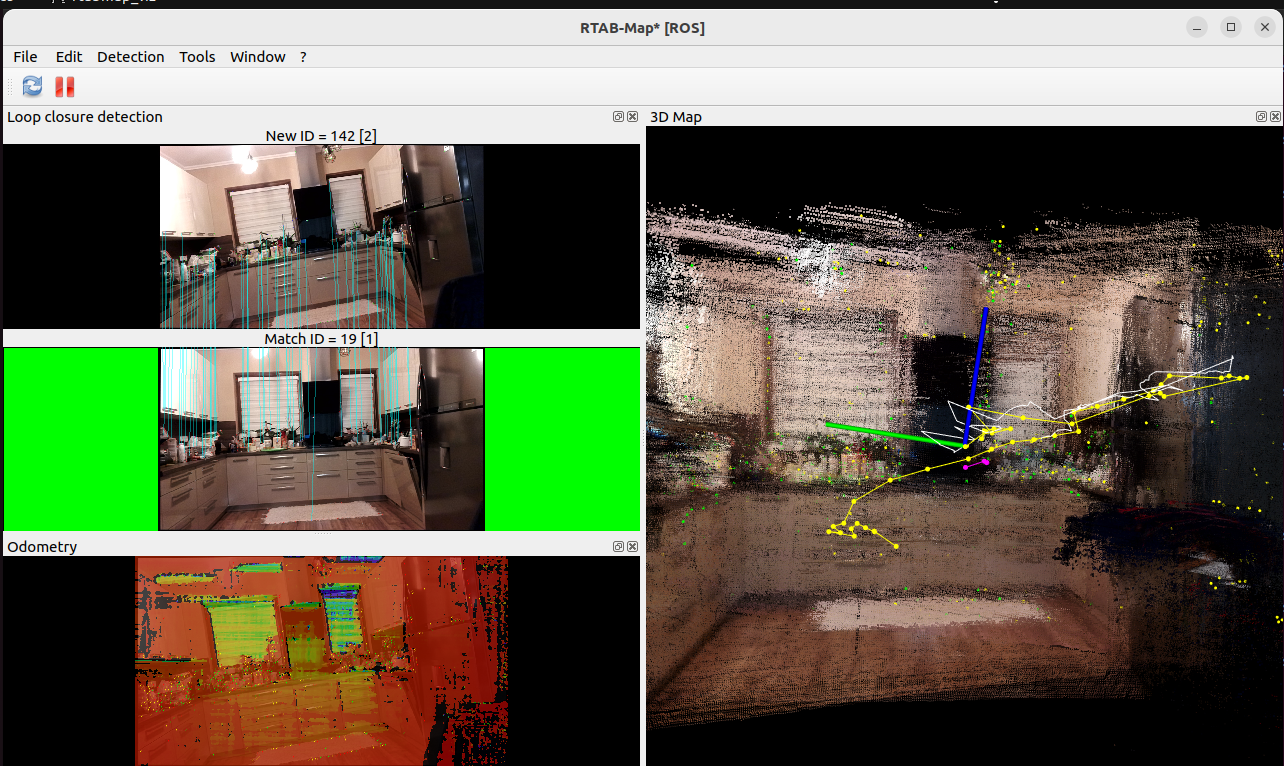
\includegraphics[width=150mm, keepaspectratio]{figures/rtabmap_ros.png}
	\caption{RTAB-Map ROS2}
	\label{fig:rtabmap_ros}
\end{figure}

One of the main limitations we encountered is RTAB-Map’s tendency to lose orientation; in such cases, the last known position is shown in the bottom-left panel, and mapping halts. To resume mapping, we must navigate back to this exact location, which is often challenging, particularly in low-light environments. Moreover, returning to the last known position did not always restore tracking, forcing us to restart the mapping process entirely. Another drawback is the latency in the camera feed, which slows down the overall process significantly.

To optimize RTAB-Map for our setup, we modified its launch files to better manage the split between the robot and a notebook on top. Ideally, the camera (mounted on the robot) should send images and IMU data over a ROS topic for processing on the notebook, which has the necessary computational resources for RTAB-Map.

By default, launching \verb|rtabmap.launch.py| from the \verb|depthai_ros_driver| package starts both the camera and RTAB-Map nodes, which was unsuitable for our setup. We needed the camera node to run on the robot and RTAB-Map on the notebook. Our solution was to create a custom launch file (details in Appendix \ref{rtabmap_custom_launch_file}) based on \verb|rtabmap.launch.py|, which excludes the camera node. Using this setup, we could launch the camera separately on the robot using \verb|camera.launch.py| from \verb|depthai_ros_driver|, while running RTAB-Map on the notebook. A map generated with this method is shown in Figure~\ref{fig:rtabmap_nokia}.

In summary, RTAB-Map’s limitations in orientation tracking and the lagging camera feed made it challenging to create detailed maps, even in small environments. Figure~\ref{fig:rtabmap_nokia} highlights that numerous irrelevant points were added to the map due to frequent orientation losses. On the actual robot, this issue was exacerbated by its high angular speed, causing repeated loss of tracking and requiring significant time and effort to recover.

\begin{figure}[htbp]
	\centering
	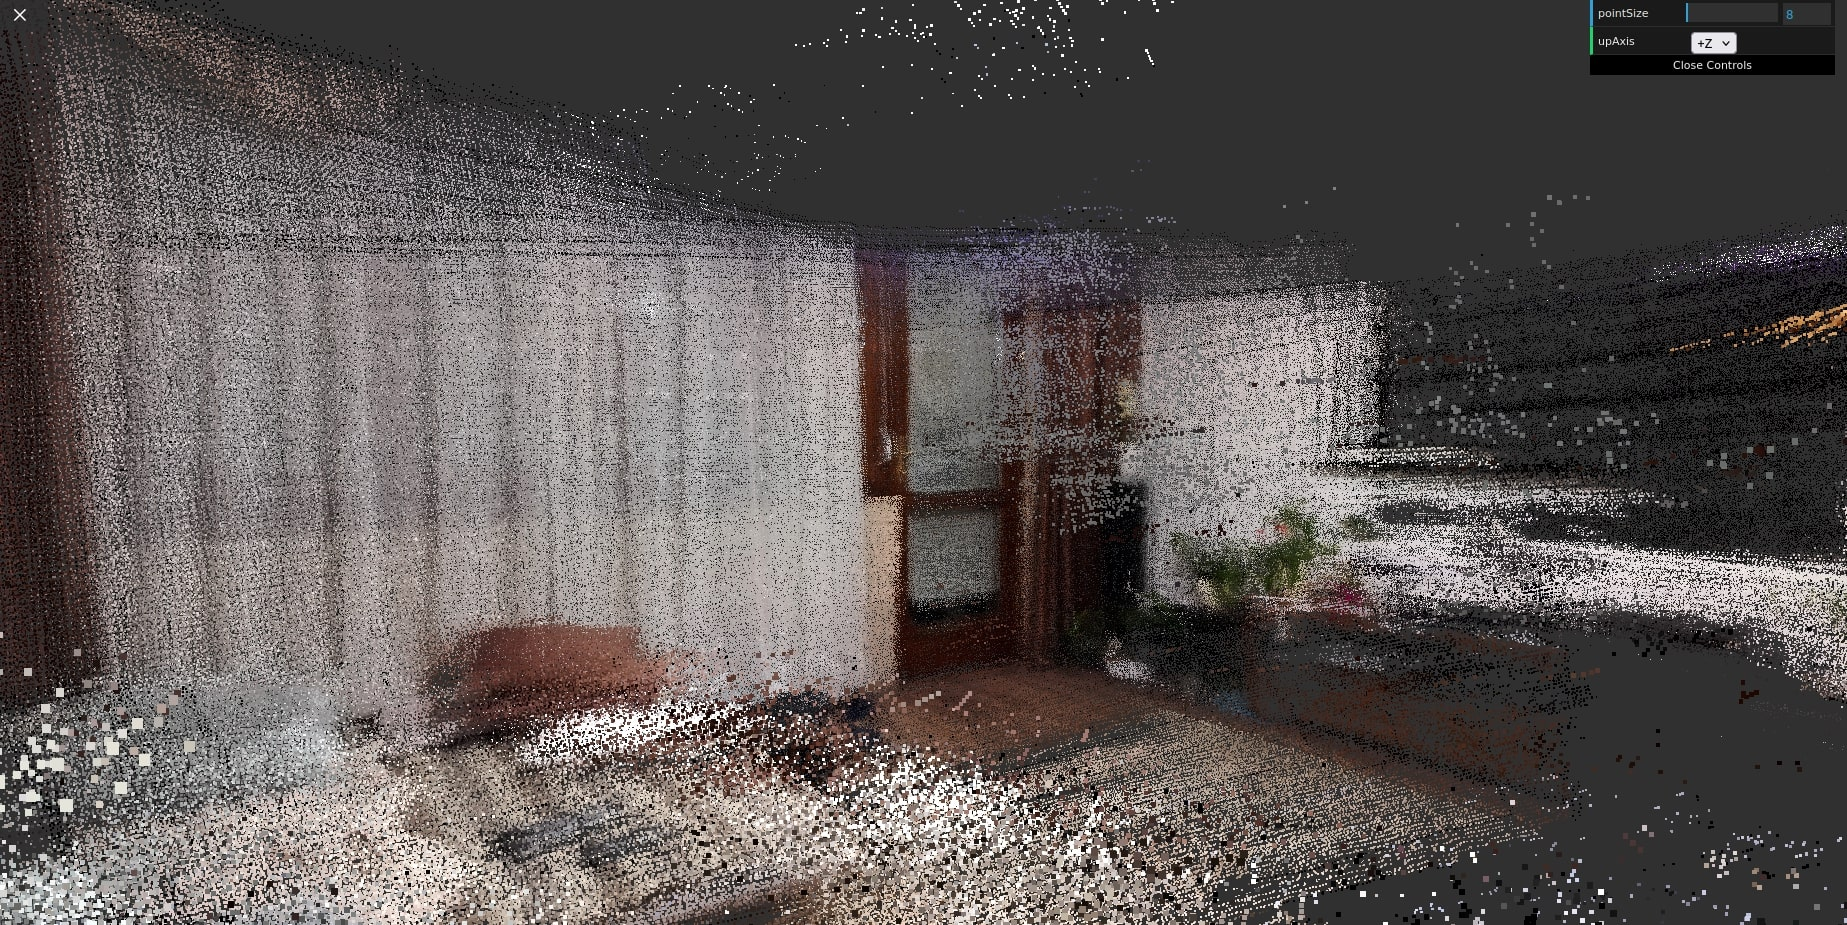
\includegraphics[width=150mm, keepaspectratio]{figures/rtabmap_ros_home.png}
	\caption{RTAB-Map ROS-generated point cloud map of our living room, camera held by hand}
	\label{fig:rtabmap_nokia}
\end{figure}

\FloatBarrier
\section{RTAB-Map iOS Application}

Out of curiosity, we also tested the iOS version of RTAB-Map and found it performed significantly better than the ROS version with the OAK-D camera. Using the same iPhone 13 Pro, I obtained a detailed reconstruction of my apartment, as shown in Figure~\ref{fig:rtabmap_ios}. This app can generate both mesh and photorealistic maps of indoor environments, operating smoothly without lag and maintaining tracking even in low-light conditions. Figure~\ref{fig:rtabmap_ios} shows a mesh map generated by the iOS app.

\begin{figure}[htbp]
	\centering
	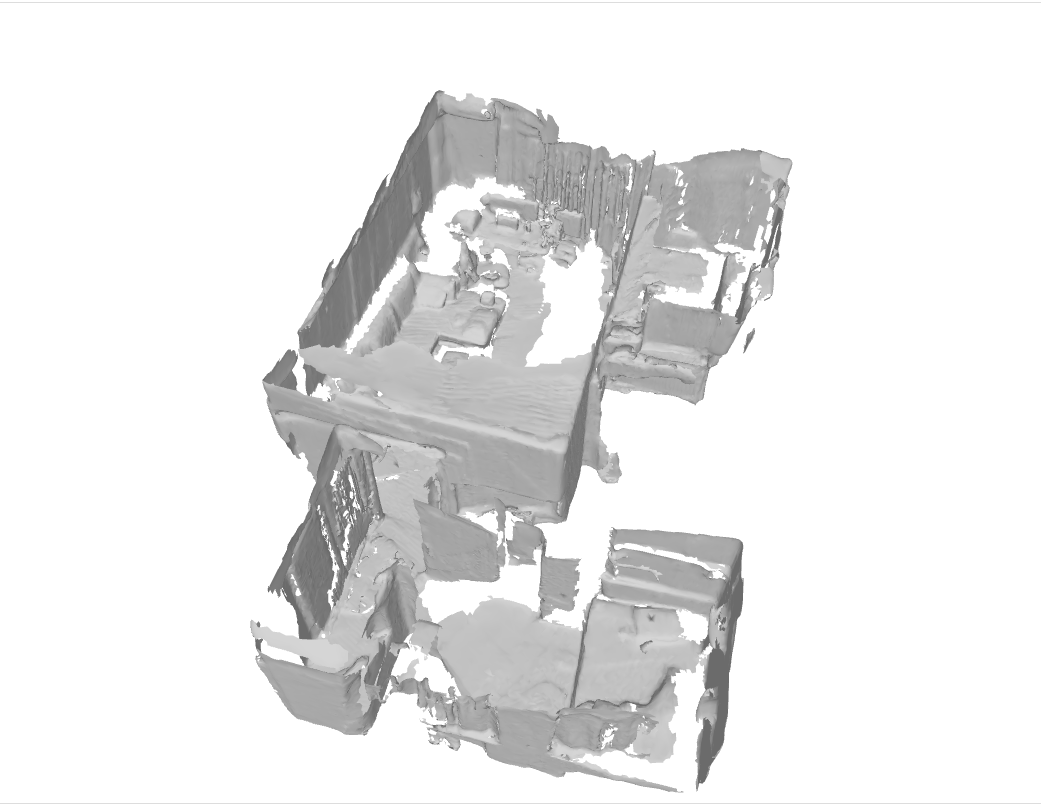
\includegraphics[width=150mm, keepaspectratio]{figures/rtabmap_ios.png}
	\caption{RTAB-Map iOS generated mesh map}
	\label{fig:rtabmap_ios}
\end{figure}
\FloatBarrier

Some visible gaps in the floor area are due to light reflections from the dark brown laminate, which created a high-contrast region that RTAB-Map could not accurately interpret, resulting in unrecognized areas on the map.


\section{Nvblox}

To begin using nvblox, I installed its dependencies and started the provided Docker container. However, when attempting to run the example code, I encountered frequent crashes. This was due to nvblox’s requirement for a minimum of 8 GB of VRAM, while my notebook, equipped with a GTX 1660 Ti GPU, only has 6 GB. Occasionally, the example did run successfully, as shown in Figure~\ref{fig:nvblox_example}. In this figure, you can observe how nvblox generates a voxel map by combining data from color and depth images along with LIDAR inputs, producing a comprehensive spatial map.

\begin{figure}[htbp]
	\centering
	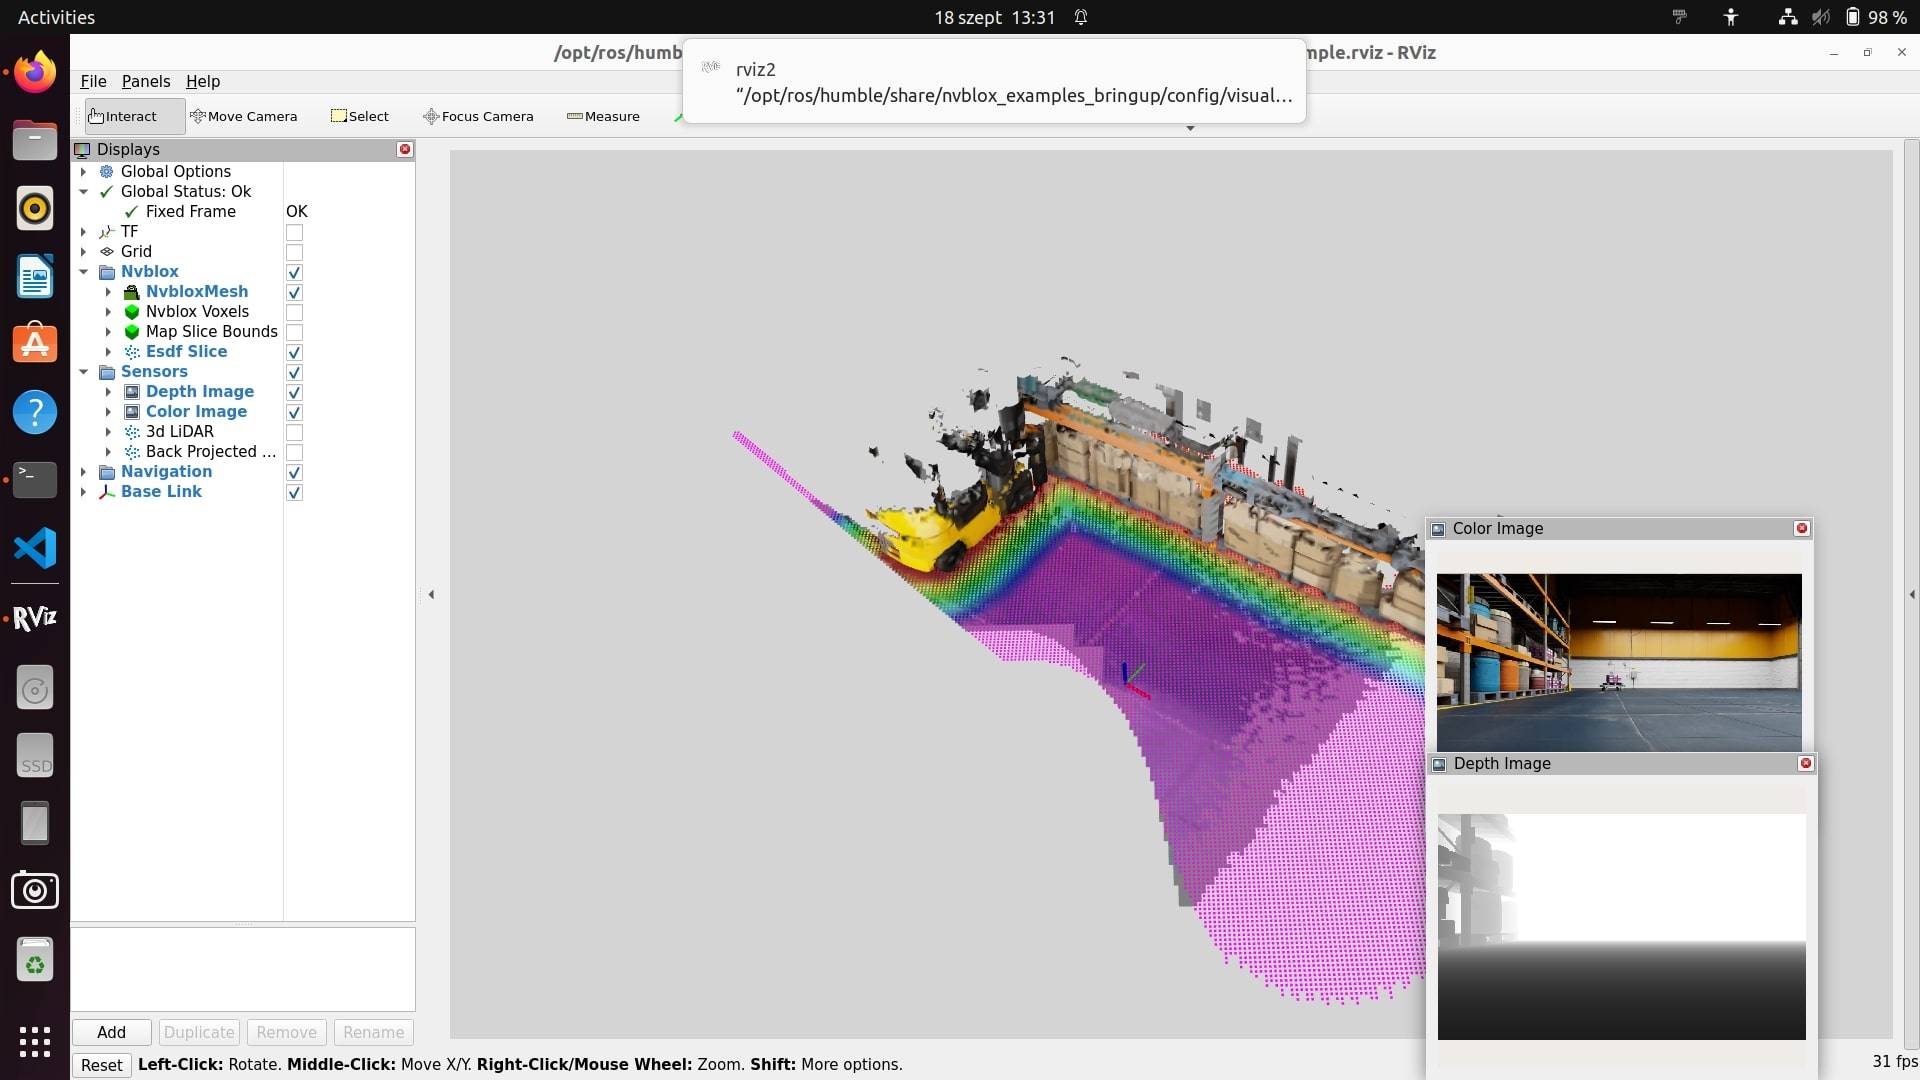
\includegraphics[width=150mm, keepaspectratio]{figures/nvblox.png}
	\caption{Running nvblox example}
	\label{fig:nvblox_example}
\end{figure}

Following my experiments with nvblox, I explored NVIDIA's Isaac VSLAM, an advanced SLAM tool that leverages NVIDIA GPUs to perform stereo visual inertial odometry (SVIO). We anticipated that Isaac VSLAM would be beneficial because it aligns well with the capabilities of the OAK-D cameras, which also support SVIO. Isaac VSLAM outputs data that can be combined with wheel odometry and LIDAR inputs, producing highly accurate localization data for ROS2's Nav2 navigation framework. Figure~\ref{fig:isaac_vslam_example} shows the Isaac VSLAM example in action. To test the Isaac VSLAM module, I used NVIDIA's isaac-sim Omniverse simulator \cite{isaac_sim_docs}. Unfortunately, the simulation environment failed to render visuals because Omniverse requires an RTX GPU to handle its advanced rendering features, which my GTX GPU could not support.

\begin{figure}[htbp]
	\centering
	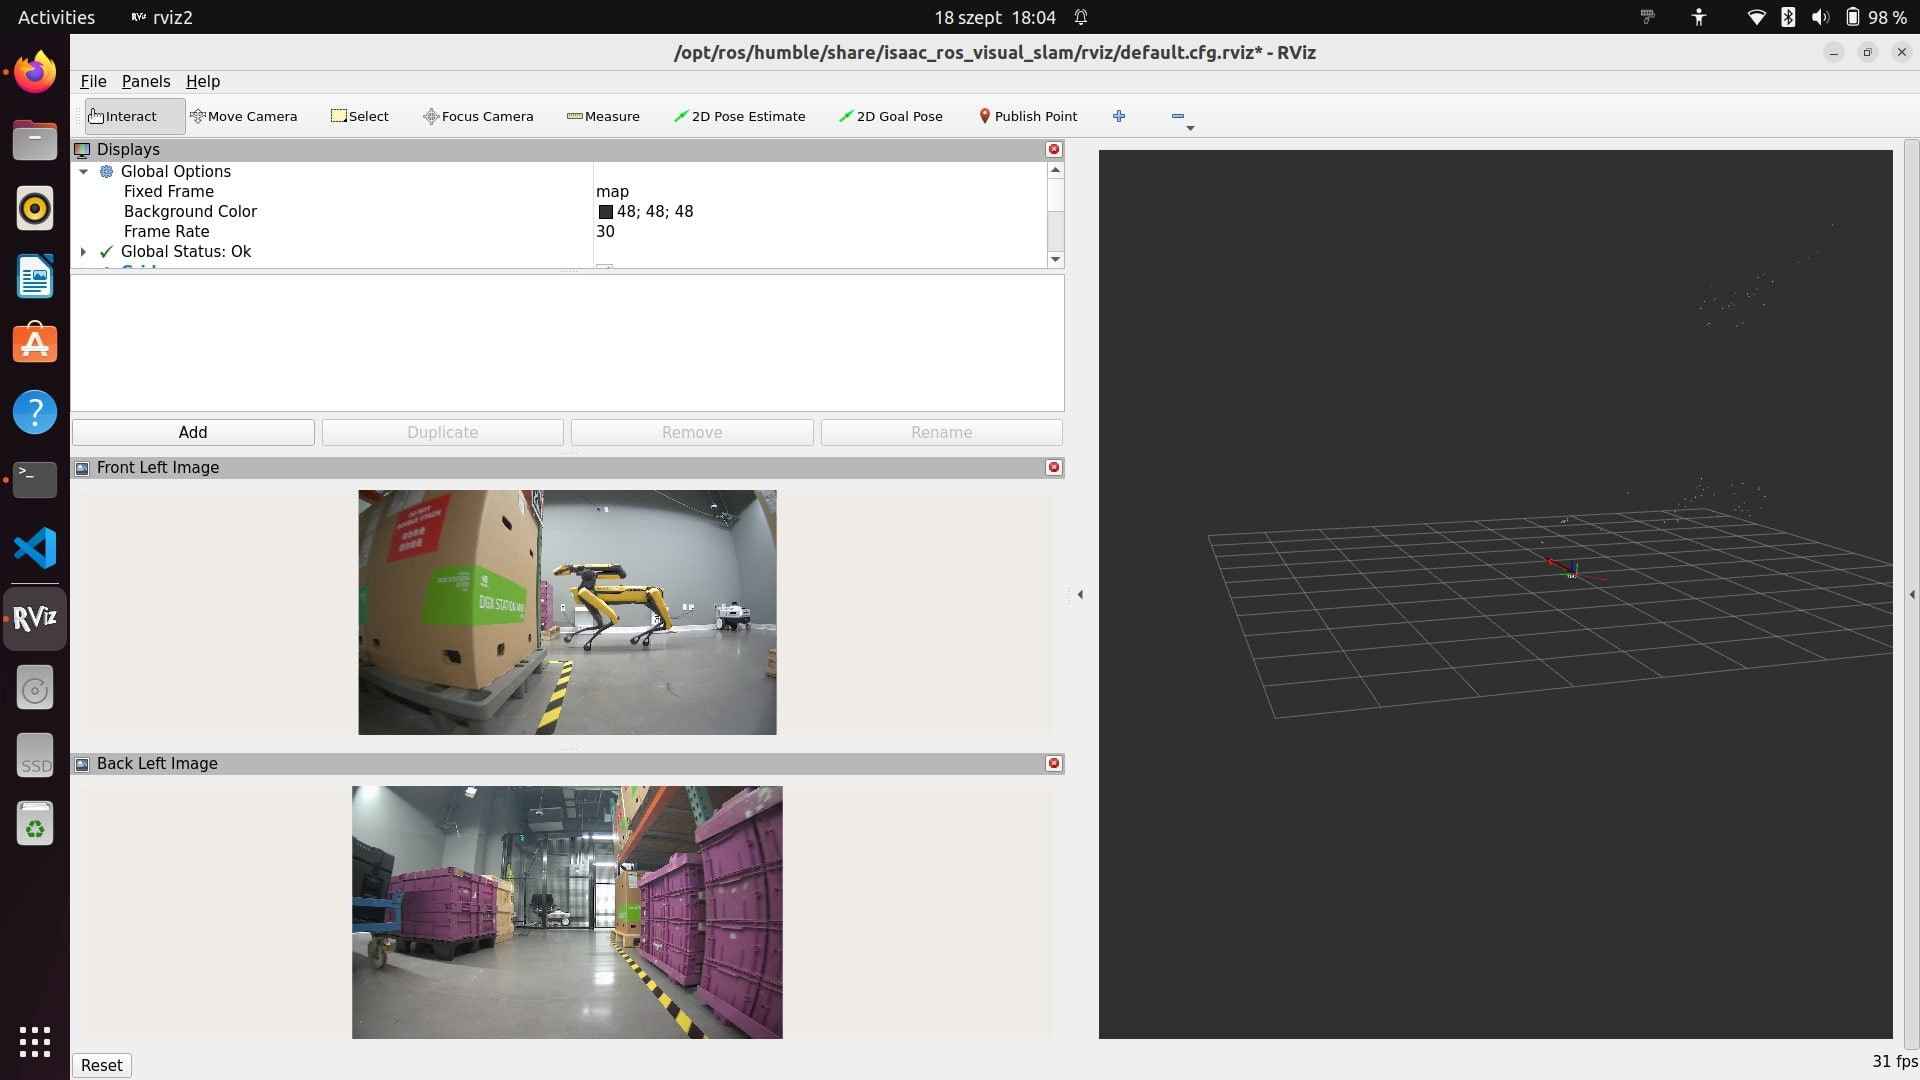
\includegraphics[width=150mm, keepaspectratio]{figures/isaac_vslam_example.png}
	\caption{Running Isaac VSLAM example}
	\label{fig:isaac_vslam_example}
\end{figure}

In the end, we opted not to use NVIDIA Isaac on the Turtlebot4 robot due to its GPU-intensive algorithms, which require at least an 8 GB VRAM-equipped Jetson module. Our robot was equipped with a Raspberry Pi 4, and we decided against investing in a Jetson due to the additional cost, which we deemed impractical for this project.
